\subsection{Implementatie Frontend}
Het laatste deel van de afstudeer applicatie is de klant zijn webstie.
Deze website moet de data van de PoC-CMS-API kunnen renderen.
Er is voor gekozen om een site na te bouwen om te kunnen kijken hoeveel maatwerk het kost om tot een mooi product te komen.
De site die hier voor gekozen is de Snakewae site (Snakeware.com).
Dit is gedaan omdat de developers van de site kan aanspreken voor mogelijke onderstuening.
Verder is de repository beschikbaar gesteld, hierdoor kunnen de exact zelfde assets gebruikt worden.
De gemaakte website (doormiddel van het afstudeer product) is te zien in figuur \ref{fig:Frontend}.


\whitespace
\begin{graphic}
    \captionsetup{type=figure}
    \caption{Frontend}
    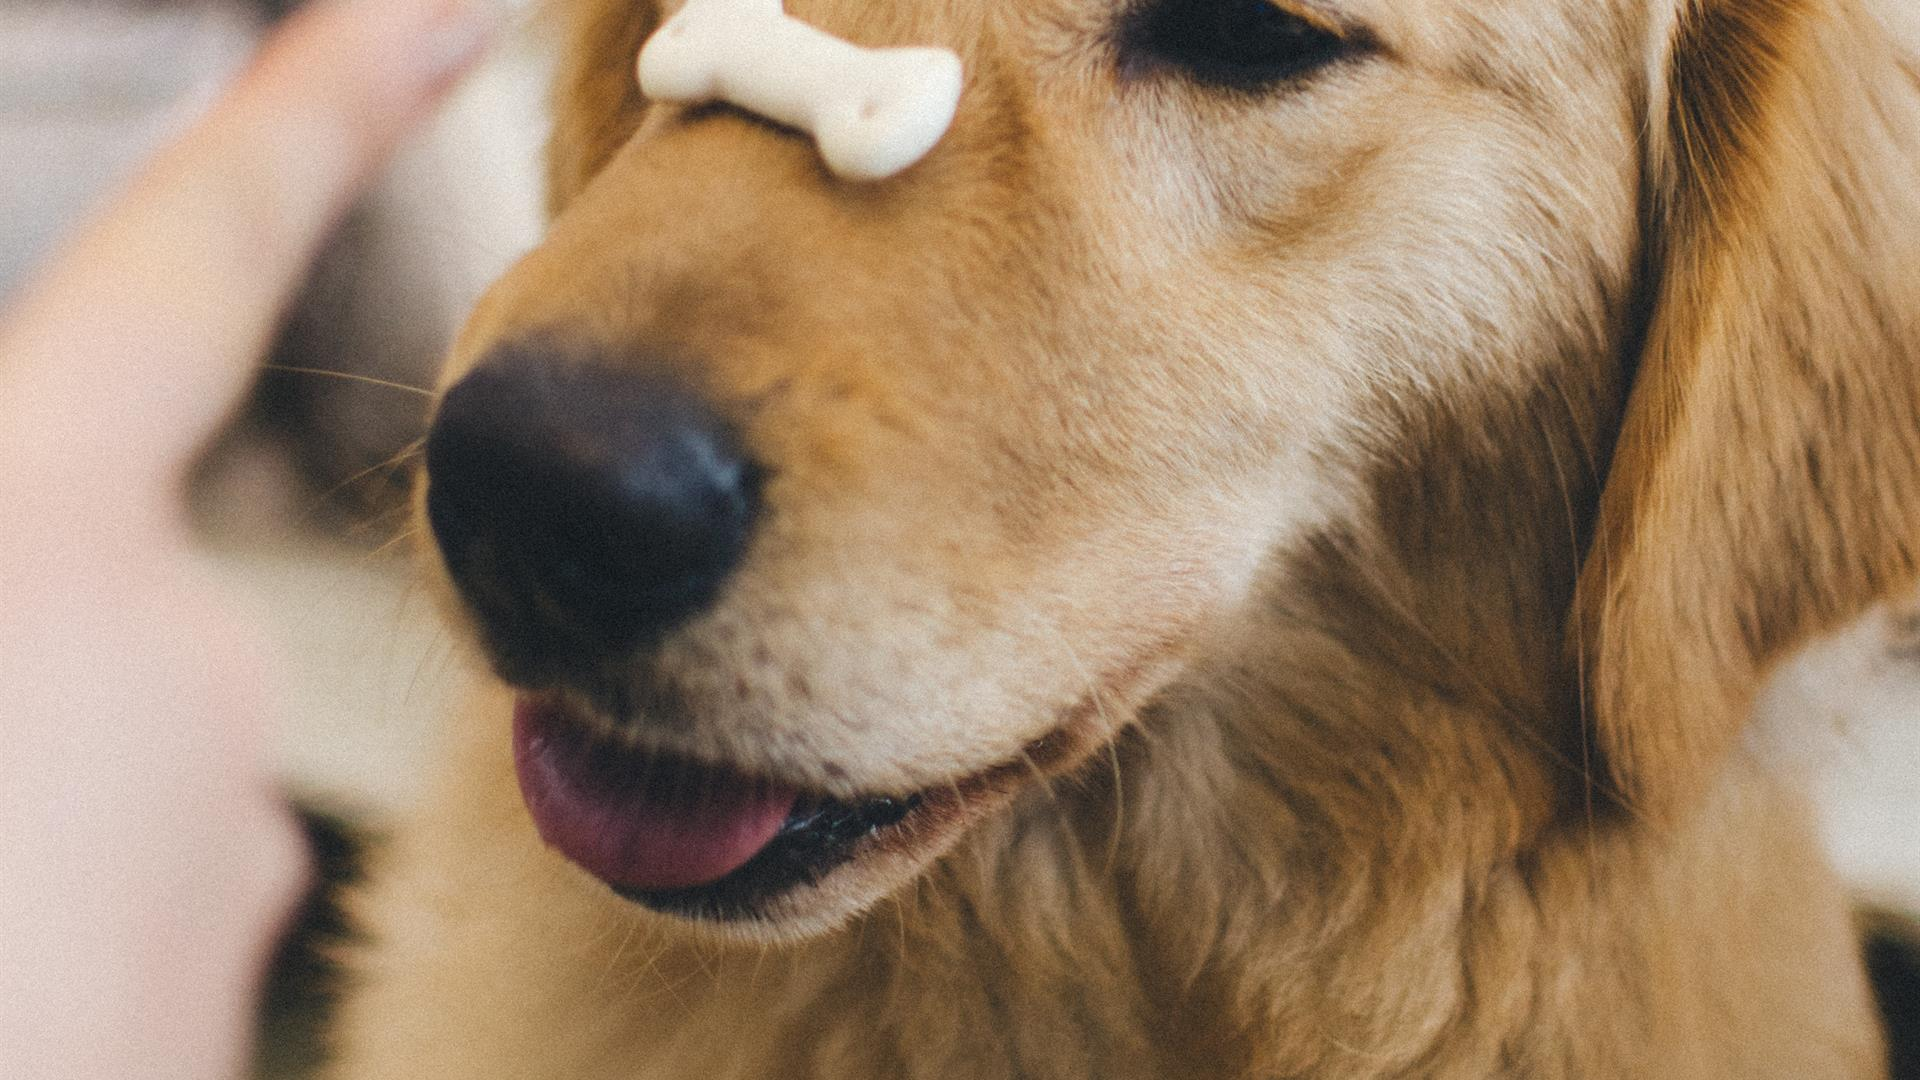
\includegraphics[scale=0.3]{Placeholder.jpg}
    \label{fig:Frontend}
\end{graphic}
